\chapter{Interferometry}
\label{chap:interferometry}

\section{Brief Overview}
\label{sec:brief-overview}

An interferometer is any device which superimposes the waves from a coherent 
light source in order to gain information about the source itself. So what does 
that mean? Let's look at the most basic case of a Michelson interferometer. In 
this scenario, we have a coherent light source (typically a laser) pointing at 
a beam splitter. The splitter splits the light into two identical beams, which 
travel on separate paths, until they are recombined before entering a detector. 
The difference in the paths creates a phase difference between the beams. This 
phase difference is what creates an interference pattern, which is what then 
gives us the information we seek about the light source, which typically comes 
in the form of fringes. 

What if instead of using mirrors and beam splitters, we built two identical 
small telescopes that were physically separated in space, then pointed them at 
the same astronomical source. Because they're not in the same spot but are 
separated by a ``baseline", there must be a difference in the path lengths 
between the telescopes and the source. This is the fundamental idea behind 
radio interferometers. Now let's explore the mathematics.

In order to get a handle on the mathematics and theory behind astronomical 
interferometry, we're going to make some simplifying assumptions. We will 
consider the case of a two-element interferometer (that is, an interferometer 
with two antennas and one ``baseline" between them) observing a very distant 
source (so the emissions from the source will come in the form of plane waves 
and the antennas will point in the same direction on the sky).  This 
interferometer will be fixed in space - so, no rotation or motion of the 
antennas themselves.  We will also be looking at just one frequency, so the 
signals coming in will be perfectly sinusoidal with one known wavelength.  We 
won't be worrying about anything in the backend, so we'll say that we have no 
frequency conversions (an RF interferometer) with a single polarization and 
perfectly idealized electronics (perfectly linear, no amplitude or phase 
distortions, perfectly identical for both instruments, and no added noise).  
We'll also assume no propagation distortions, so the plane waves we observe 
from the source won't be disturbed by the ionosphere or atmosphere of Earth, 
and that the source is small enough in angular size that we can approximate the 
sky as flat and two-dimensional. 

What does that leave us? Two identical sensors that are separated by a vector 
distance $\mathbf{b}$ - this is our baseline. These sensors are both pointed at 
a quasi-monochromatic source of frequency $\nu$, in the vector direction 
$\mathbf{s}$.  Combining these fundamental numbers, we then get the key 
quantity $\tau_g = \mathbf{b} \cdot \mathbf{s} / c$, which is the geometric 
time delay. That's the extra time needed for the signal to reach the more 
distant antenna. This number will be important to us in order to correlate our 
signals.  We can also find the phase shift in the signal by writing $\Theta = 
\omega \tau_g = 2 \pi \mathbf{b} \cdot \mathbf{s} / \lambda$.

With this knowledge of the phase difference between the paths, we can write out 
the voltages received by each of the sensors, so we get $V_1 = E \cos{[\omega(t 
- \tau_g)]}$, because it has that extra phase delay from the baseline 
separation, and $V_2 = \cos{(\omega t)}$. In this case, the path lengths from 
the sensor to the multiplier are treated as being equal, so we don't need to 
add any extra phase terms. We then multiply our signals together, and take an 
average over time, which gives us an averaged product $R_C = P \cos{(\omega 
\tau_g)}$. This quantity is dependent on the received power $P = E^2/2$ and the 
geometric delay $\tau_g$, and hence on the baseline orientation and source 
direction. We can rewrite $R_C$ to make this relationship more explicit as:

\begin{equation}
    R_C = P \cos{(2 \pi \frac{\mathbf{b} \cdot \mathbf{s}}{\lambda})}
    \label{eq:R_C}
\end{equation}

Note that $R_C$ is not a function of the time of the observation (so long as 
the source itself is not transient or variable), the physical location of the 
baseline (provided that the source is in the far field, which is always true of 
astronomical sources), or the actual phase of the incoming signals.  All that 
matters is the relative phase between the sensors!

In order to get a better understanding of our observed response, let's rewrite 
some terms. Let us say that $\mathbf{b} \cdot \mathbf{s}/\lambda = 
u\cos{\alpha} = u\sin{\theta} = ul$. In this case, we are defining 

\begin{equation}
    u \equiv b/\lambda
    \label{eq:u}
\end{equation}

\noindent which is the baseline length in units of wavelengths, and $\theta$ is 
the angle relative to the zenith. $l = \cos{\alpha} = \sin{\theta}$ is the 
direction cosine. We can then rewrite our response function as $R_C = P \cos{(2 
\pi ul)}$. We can now see quite easily that the longer the baseline, the more 
rapid the frequency of the response function $R_C$. This is what radio 
astronomers call ``fringes".

We can also begin to see why we want to have many sets of antennas - each 
baseline will only give us information about one set of fringes. In order to 
reconstruct a full image of an extended source, we need to be able to observe 
more than one spatial frequency. The response from an extended source is 
obtained by summing the responses at each antenna to all emission over the sky, 
multiplying the two for each pair of antennas, and averaging. Assuming that the 
source itself is spatially incoherent (e.g. that the emission from one side of 
the galaxy isn't related to the emission from the other side), the averaging 
and integrals can be interchanged, giving us

\begin{equation}
    R_C = \iint I(\mathbf s) \cos(2\pi\nu\mathbf{b}\cdot\mathbf{s}/c) d\Omega
    \label{eq:even-response}
\end{equation}

We can now see the relationship between what we are measuring to what we want 
to observe - we have linked the source brightness $I_\nu(\mathbf{s})$ to the 
even interferometer response $R_C$. To complete the image of the sky, we can 
observe the odd interferometer response $R_S$, which is the sinusoidal 
equivalent of $R_C$, by slipping in a $90^{\circ}$ phase offset along one of 
the signal paths.   

Now we can define a complex function $V = R_C - iR_S = A e^{-i \phi}$ as our 
complex visibility from the two independent, real correlator outputs $R_C$ and 
$R_S$, where $A = \sqrt{R_C^2 + R_S^2}$ and $\phi = \tan^{-1}{(R_S/R_C)}$.

We can now rewrite the complex visibility as an integral, giving us:

\begin{equation}
    V(\mathbf{b}) = R_C - iR_S = \iint I(\mathbf s) e^{-2\pi i 
    \nu\mathbf{b}\cdot\mathbf{s}/c} ~d\Omega
    \label{eq:vis}
\end{equation}

This is easily recognized as the 2D Fourier transform, when the right geometry 
is utilized. As it turns out, the earlier definitions of $u$ and $l$ are very 
convenient coordinates to use, and can be expanded to two dimensions to give us 
the $(u,v)$ visibility plane and the $(l,m)$ source plane\footnote{In 
actuality, we don't use the $uv$-plane, but rather calculate from baselines 
$\mathbf{b}$ and source direction $\mathbf{s}$ directly, so as to avoid any 
complications or imprecision due to usage of the flat-sky approximation. See 
Appendix~\ref{appendix} for more information on the $uv$-plane and when it is 
an appropriate coordinate system to use.}.  

Additionally, so far we have avoided mentioning any frequency dependence in 
this relationship or any intrinsic instrumental effects. The fact of the matter 
is that every astronomical array will have a frequency dependence, either from 
the response of the instrument itself or from the changing physics of the 
visible celestial sky (or, more likely, both). Therefore we must in fact 
calculate visibilities for all the frequencies within our science band (i.e.  
for each channel, meaning that there will be a level of imprecision and 
integration of each visibility across a known $\delta \nu$ of frequency space 
in the science band).

Moreover, we must also account for the fact that no antenna has perfect 
reception to the entire sky -- rather, each antenna has some spatial 
sensitivity related to its own shape. This shape is often referred to as the 
``beam" or the ``primary beam" of the antenna, and we shall denote it as 
$A(l,m)$. 

Eq.~\eqref{eq:vis} can now be rewritten with these coordinates like so:

\begin{equation}
    V_\nu(u,v) = \iint I'_\nu(l,m) e^{-2\pi i (ul + vm)} ~dl ~dm
    \label{eq:van-cittert}
\end{equation}

\noindent where $I'_\nu(l,m) = I_\nu(l,m) A_\nu(l,m)$. This is the van 
Cittert-Zernike theorem, a fundamental equation for interferometry, which 
relates the brightness of the distant source to the mutual coherence function 
(or visibility) via the 2D Fourier transform in a convenient set of coordinates 
for radio astronomy.

\section{Spatial Modes and Interferometric Sensitivities}

As mentioned above in Section~\ref{sec:brief-overview}, interferometry gives 
you sensitivity to different spatially varying modes based on the physical 
separation of the antennas or telescope reflecting dishes making the 
observation. The bigger the separation, the faster the spatial variation 
observed on the sky, and therefore the higher resolution/smaller the object 
that can be observed.

It is through this knowledge that we are able to construct instruments that are 
specifically tuned to different spatial scales. For example, astronomers (and 
the general public) are fascinated by black holes and want to observe their 
inner workings. Black holes are very compact objects in the sky, so to be able 
to resolve them takes incredibly high resolution observations. Under the 
Rayleigh criterion (Eq.~\ref{eq:rayleigh}), radio astronomers can achieve fine 
resolution (i.e. small $\theta$)  by using high frequencies (i.e.  small 
$\lambda$, of the order of less than a millimeter) and very large baselines 
(i.e.  large $B$, on the order of thousands of kilometers).

\begin{equation}
    \theta = \lambda / B
    \label{eq:rayleigh}
\end{equation}

Alternately, if one wanted to observe fluffy galactic clouds or other extended 
structures, they would instead prefer to construct an interferometer using 
closely packed antennas and lower frequencies.

By constructing an array using a combination of differing baselines, one can 
fill in the sampling of the $uv$-plane. With complete sampling of the $uv$-
plane, one can perform a simple 2D Fourier transform and perfectly recreate the 
image plane. This relationship between spatial frequency and images, or 
visibility and brightness, is known as the \emph{spatial Fourier transform}, 
and is the backbone of all radio interferometry, from the reconstruction of 
cosmological power spectra all the way to the sophisticated synthesis imaging 
techniques described above.

In reality, of course, it is impossible to completely sample the $uv$-plane and 
recover a perfect image. We must therefore design our instruments to be 
maximally effective at the observations we wish for them to make. In the cases 
of general purpose instruments like the Very Large Array (VLA), that means 
designing the instrument to be very flexible -- covering a broad range of 
frequencies, minimizing redundancy in the baselines, and using different array 
configurations to better sample different regions of the $uv$-plane.

However, for smaller scale instruments, astronomers generally wish to build 
something which is very specifically tailored for the observation they want to 
be making, leading to creative and highly unique array configurations that make 
use of the spatial Fourier transform to the best of their ability.

\subsection{Spatial Fourier Transforms}

Much as we can think of the relationship between time and frequency as a 
Fourier pair, we can also relate the physical separation of the antennas (i.e.  
the ``geometric time delay" $\tau_g$) and the spatial frequency.

Consider the variable $u$, which is defined as the baseline separation of two 
antennas measured in wavelengths in Eq.~\eqref{eq:u}.  Based on 
Eq.~\eqref{eq:R_C}, we also know that $R_C \approx \cos(2\pi u l)$, meaning 
that the number of whole fringes imposed across the sky for any given 
separation will be $N_f = 2u$. 

This in turn means that a pair of antennas separated by $u$ wavelengths will be 
most sensitive to objects with an angular scale of about $\theta = 1 / u$, 
according to Eq.~\eqref{eq:rayleigh}.

One can relate this to the idea of spherical harmonics, with the harmonics 
providing us the $(l,m)$ coordinates of our observed brightness, providing us 
some context for the second member of our spatial Fourier pair. We can thus 
start visualizing the physical meaning of ``spatial variance" and ``spatial 
frequencies".

We can do so by rewriting our interferometric visibility in terms of spherical 
harmonics. Let's begin by rewriting our visibility equation into the form seen 
in Eq.~\eqref{eq:vis}, now factoring in the primary beam and integrating over 
the full celestial sphere.

\begin{equation}
    V(\nu) = \int I(\mathbf s) A(\mathbf{s}) e^{-2\pi i 
    \nu\mathbf{b}\cdot\mathbf{s}/c} ~d\mathbf{s}
    \label{eq:vis-allsky}
\end{equation}

\noindent where $I(\mathbf{s})$ is the sky brightness, $A(\mathbf{s})$ is the 
primary beam of the antenna, and the exponential term is the interferometric 
``fringe".  Now, much in the way that any signal can be decomposed into an 
infinite series of Fourier frequencies and amplitudes, we can rewrite the terms 
of Eq.~\eqref{eq:vis-allsky} to be expressed as a sum of spherical harmonics.

\begin{equation}
    I(\mathbf s) = \sum_{l,m} I_{lm} Y_l^m(\mathbf{s})
    \label{eq:sky-spherical-harmonics}
\end{equation}

\noindent and therefore the visibility equation becomes:

\begin{equation}
    V(\nu) = \int \Big( \sum_{l,m} I_{lm} Y_l^m(\mathbf{s}) \Big) A(\mathbf{s}) 
    e^{-2\pi i \nu\mathbf{b}\cdot\mathbf{s}/c} ~d\mathbf{s}
    \label{eq:vis-allsky-lm}
\end{equation}

So now the question is simply: does the integral of the zeroth mode (i.e. the 
global signal) vanish or not. This term can be written as:

\begin{equation}
    V_0(\nu) \equiv I_{00}(\nu) \int Y_0^0(\mathbf{s}) A(\mathbf{s}) e^{-2\pi i 
    \nu\mathbf{b}\cdot\mathbf{s}/c} ~d\mathbf{s}
    \label{eq:vis-allsky-00}
\end{equation}

We know that $Y_0^0 = \sqrt{1/4\pi}$, so the remaining question of interest 
basically boils down to whether or not the beam can break the inherent symmetry 
of the fringe term, leaving us with a non-zero $V_0(\nu)$.

%ROPE IN TOP HAT-BESSEL DUALITY HERE -- WHAT IF BEAM IS A TOP HAT? SHOW SOME 
%EQUATIONS

\begin{figure}
    \begin{center}
    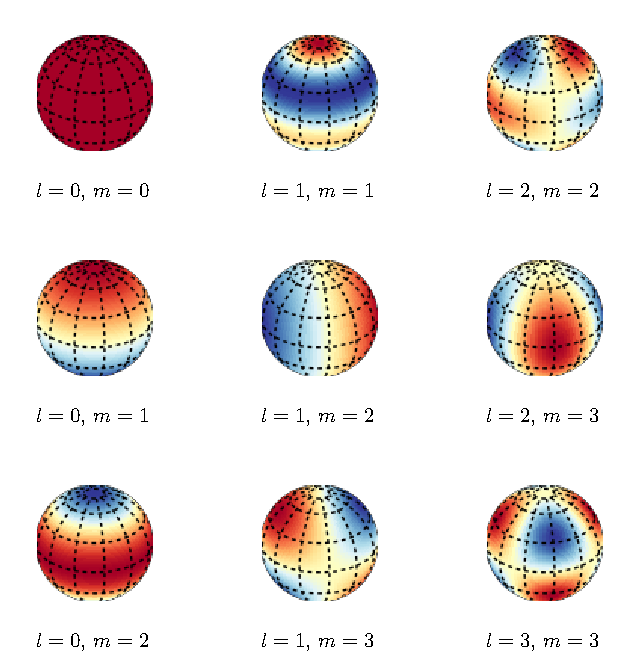
\includegraphics[width=\linewidth]{spherical_harmonics}
    \end{center}
    \caption{
         Above, we see a collection of the low-order spherical harmonic 
         functions. This can help us begin to visualize what, physically, the 
         spherical harmonics are and how they can be used to parse spatial 
         information observed on the sky from an interferometer.
    }
    \label{fig:spherical-harmonics}
\end{figure}

\section{Observing the Spatial Monopole with an Interferometer}
\label{sec:observing-monopole}

At this point, it is a fair enough question to ask how exactly we intend to use 
an interferometer to observe a spatially invariant signal. Everything we have 
stated above indicates that interferometers see \emph{changing} signals -- they 
observe the spatial variance that they are sensitive to based upon the 
separation of the antennas and the frequency they are observing at. They are 
inherently AC circuits. The one thing they are explicitly not meant to do is to 
observe what is effectively a DC tone.

Fortunately, we can make sure that we aren't actually observing a DC tone. As 
addressed in~\citet{presley2015}, we're on earth and can't actually see a 
monopole from the sky -- the horizon gets in the way.  Furthermore, the antenna 
itself has a directionally dependent beam, introducing an additional layer of 
spatial variance. Therefore, what in reality is a monopole signal from the 
entire universe is instead observed with a spatial cut-off -- it's a top-hat.  
Or, more accurately (with the addition of the primary beam $A$), it's a bowler 
hat. And, most importantly for our goals, a top-hat signal doesn't necessarily 
integrate to zero and therefore may be observable with an 
interferometer~\citep{venumadhav2016}.

That being said, a top-hat signal that spatially broad still isn't easily 
observable with an interferometer. From our knowledge of Fourier transformed, 
we know that a broad spatial cut-off translates into a narrow spread of powers 
in the visibility domain -- i.e. most of the monopole power will remain in very 
broad, long and low spatial modes. If we want to truly convert the monopole 
into a signal that we can get at with an interferometer, we're going to have to 
constrict the scale of our spatial top hat.

What we need to do is artificially push our monopole term into higher modes -- 
modes that we are in control of. Or, in Fourier terminology, we need to apply a 
top-hat function to our monopole signal. 

In doing so, we will generate a visibility sensitivity in the shape of a sinc 
function -- meaning we will have sensitivity to our monopole term in many 
Fourier modes, rather than just in the $(0,0)$ or $(0,1)$ modes. If we control 
the shape of the top hat imposed, then we know the shape of the sinc function, 
meaning we can calibrate exactly what our monopole sensitivity should be at any 
given point in the $uv$-plane.

\begin{figure}
    \begin{center}
    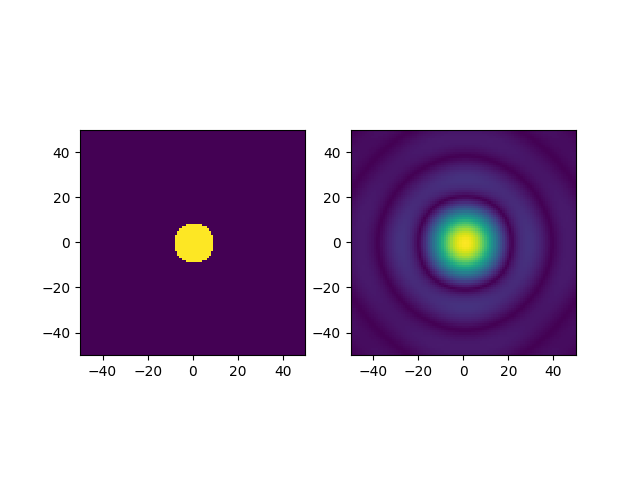
\includegraphics[width=\linewidth]{top-hat-bessel.png}
    \end{center}
    \caption{
        This figure shows the Fourier relationship between the two-dimensional 
        top hat function and a Bessel function. This image can be thought of as 
        an idealized cartoon of the aperture and visibility planes of our 
        proposed interferometer. On the left, we see the imposed top-hat, where 
        the yellow portion would be the portion of monopole sky visible to the 
        antenna and the blue would be the perfect absorber. On the right, we 
        have performed a two-dimensional Fourier transform to convert into the 
        visibility plane (i.e. to see the spatial modes to which we are 
        observationally sensitive), and we see this rippling function centered 
        around the zero-spacing mode.
    }
    \label{fig:sinc}
\end{figure}

So now the question is simply how can we raise the horizon that our antennas 
see? One option would be to literally raise the horizon -- either find or 
manufacture a deep valley for them to reside within. This would probably be 
challenging to do well -- digging a valley for the whole array would 
undoubtedly be expensive, and it'd be very hard to find a naturally occurring, 
rotationally symmetric valley (particularly one deep enough to actually 
meaningfully raise the horizon of our antennas).

So we must find a way to artificially raise the horizon of our antennas.  
Moreso, as described in~\citet{venumadhav2016}, we must either allow our 
antennas to freely cross-talk (thereby eliminating the vast majority of 
benefits gained from using an interferometric setup) or we must introduce a 
source of noise from lossy components (e.g. the ground or other signal 
absorbers, rather than reflectors or transmitters) in order to maintain a 
sensitivity to the global signal. As described in 
Section~\ref{sec:brief-overview}, the more closely spaced your elements, the 
larger the spatial scales on the sky your instrument will be sensitive to. We 
therefore know that we are going to be using a very closely packed array, which 
will make our system very prone to cross-talk. If we want to avoid that, then 
we'll have to find some way to ensure that the antennas don't see each other in 
addition to seeing less of the sky.

All of which leads us to the construction of thin absorptive walls between the 
antennas -- introducing a new horizon in how the antenna sees the sky and 
maintaining the independence of each antenna's signal from its very nearby 
neighbors. In order to maximize our sensitivity to the global signal, we will 
want the absorbers used to be highly efficient at dissipating energy across our 
frequency spectrum~\citep{venumadhav2016}. This will provide us will a strong 
``edge" in how our antennas see the sky, in turn creating maximal Fourier 
leakage into higher modes and best enabling us to make a successful observation 
of the reionization monopole signal.
